\documentclass[11pt, preprint]{aastex}
%%%%%%begin preamble
\usepackage[hmargin=1.05in, vmargin=1in]{geometry} % Margins
\usepackage{hyperref}
\usepackage{url}
\usepackage{natbib}
\usepackage{graphicx}
\usepackage{amsmath}
\usepackage{amsfonts}
\usepackage{amssymb}
\usepackage{pdfpages} % breaks with aastex6
\usepackage{import}
\usepackage{wrapfig}

\usepackage{color}
\hypersetup{
  colorlinks   = true,
  %citecolor    = blue
  citecolor    = gray
  % gray is not being found!?!
  % gray is found if pdfpages is used... crap.
  %citecolor    = grey
  %citecolor    = Gray
}

\setcounter{tocdepth}{2}
%% headers
\usepackage{fancyhdr}
\pagestyle{empty}
\pagenumbering{gobble}
\renewcommand*{\thefootnote}{\fnsymbol{footnote}}

\renewcommand{\vec}{\ensuremath{\boldsymbol}}
\newcommand{\dedalus}{\href{http://dedalus-project.org}{Dedalus}}
\newcommand{\del}{\ensuremath{\vec{\nabla}}}
\newcommand{\scrS}{\ensuremath{\mathcal{S}}}

\newcommand{\nosection}[1]{%
  \refstepcounter{section}%
  \addcontentsline{toc}{section}{\protect\numberline{\thesection}#1}%
  \markright{#1}}
\newcommand{\nosubsection}[1]{%
  \refstepcounter{subsection}%
  \addcontentsline{toc}{subsection}{\protect\numberline{\thesubsection}#1}%
  \markright{#1}}

\usepackage{atbegshi}
%%%%%%end preamble
%
%
%
%
%\usepackage{natbib}
%\setlength{\bibsep}{0pt plus 0.3ex}
%\usepackage[margin=1in]{geometry}
%\usepackage{sectsty}
%\usepackage{graphicx}
%\usepackage{hyperref}
%\usepackage{epstopdf}
%\usepackage{anyfontsize}
%\usepackage{wrapfig}
%\usepackage[skip=2pt,font=small]{caption}
%\captionsetup{width=\textwidth}
%\usepackage{amssymb, amsmath, amsfonts, xcolor}
%\hypersetup{
%    colorlinks,
%    linkcolor={red!50!black},
%    citecolor={blue!80!black},
%    urlcolor={blue!80!black}
%}
%
%
%\sectionfont{\normalsize}
%\subsectionfont{\small}
%
%
%%\citestyle{aa}
%%\newcommand{\aj}{The Astronomical Journal}
%%\newcommand{\apj}{The Astrophysical Journal}
%%\newcommand{\apjl}{The Astrophysical Journal Letters}
%%\newcommand{\apjs}{The Astrophysical Journal Supplemental Series}
%%\newcommand{\aap}{Astronomy \& Astrophysics}
%%\newcommand{\aaps}{Astronomy \& Astrophysics Supplemental Series}
%%\newcommand{\mnras}{Monthly Notices of the Royal Astronomical Society}
%%\newcommand{\baas}{Bulletin of the American Astronomical Society}
%%\newcommand{\ssr}{Space Science Reviews}
%%\newcommand{\zap}{Zeitschrift für Astrophysik}
%\newcommand{\sol}{\ensuremath{\odot}}
%\newcommand{\RB}{Rayleigh-B\'{e}nard }
%\newcommand{\grad}{\ensuremath{\nabla}}
%
%\usepackage{fancyhdr}
%\pagestyle{fancy}
%\fancyhf{} % sets both header and footer to nothing
%\renewcommand{\headrulewidth}{0pt}
%\renewcommand{\footrulewidth}{0pt}
%%\rfoot{\footnotesize{Evan H. Anders NSF AAPF 2019}}
%%\lfoot{\footnotesize{\leftmark}}
%%%\lfoot{\footnotesize{\leftmark}}%\thesection: \sectiontitle}}
%%\cfoot{\footnotesize{\thepage}}
%
%\makeatletter
%\renewcommand{\sectionmark}[1]{%
%  \markboth{\ifnum \c@secnumdepth>\z@
%      \thesection: \hskip 1em\relax
%    \fi #1}{}}
%\makeatother
%
%\usepackage{titlesec}
%%\titleformat{\abstract}[runin]{\normalfont\normalsize\bfseries}{\theabstract}{1em}{}
%\titleformat{\section}[hang]{\normalfont\fontsize{14pt}{17pt}\selectfont\bfseries}{\thesection}{1em}{}
%\titleformat{\subsection}[runin]{\normalfont\fontsize{12.5pt}{14pt}\selectfont\bfseries}{\thesubsection}{1em}{}
%\titleformat{\subsubsection}[runin]{\normalfont\normalsize\bfseries}{\thesubsubsection}{1em}{}
%
%\renewenvironment{abstract}
%{
%\noindent \par{\bfseries \abstractname.}}
%{\medskip\noindent 
%}
%
%
%


\begin{document}
\title{Convective Conundrums in the Asteroseismic Age:\\The interplay of rotation and magnetism in stellar convection}
\maketitle
\begin{flushleft}
  \textit{Principal Investigator:} Evan H. Anders 
\end{flushleft}

\vspace{-1cm}


%\begin{center}
%   \Large\textbf{Convective Conundrums in the Asteroseismic Age: }\\
%   \Large\textbf{The interplay of rotation and magnetism in stellar convection  }\\
%   \vspace{0.2cm}
%   \large{Evan H. Anders}\\
%   \vspace{0.2cm}
%\end{center}
%
%\vspace{-0.4cm}
%
%\begin{abstract}
%The past two decades have seen an impressive rise in our understanding of the interior structure of the Sun and countless other stars through helioseismic and asteroseismic techniques.
%These observations often rely on inversions which are informed by simple models of stellar convection which do not include the important effects of magnetism and rotation.
%Furthermore, these helioseismic observations of the Sun have called into question even our most fundamental understanding of stellar convection -- a problem widely referred to as the Solar Convective Conundrum.
%Recent literature has suggested that complicating effects, such as rotation, may be the crucial pieces missing in our understanding.
%During my postdoctoral studies, I propose to study how rotation and magnetism affect the dynamics of stellar convection from the smallest to the largest scales.
%I will conduct detailed studies of individual stellar downflows and mesoscale studies of convective interactions at the radiative-convective interface.
%I will further develop community tools to decrease the computational cost of global simulations of stellar convection, enabling improved stellar models and synthetic observables.
%\end{abstract}

\vspace{-0.6cm}

\section{Motivation}
\sectionmark{Motivation}
\vspace{-6pt}

\paragraph{Asteroseismology}
\label{sct:asteroseismology}
The advent of asteroseismic science has closely paralleled that of exoplanetary science.
The earliest ground-based observations of stellar pulsations\citep[e.g.,][]{kjeldsen&frandsen1991, bouchy&carrier2001, bedding&all2001} have given way to datasets larger than $10^4$ stars \citep[e.g.,][]{yu&all2018, santos&all2019b} in the age of CoRoT, Kepler, and K2 data.
Another 20,000 asteroseismically-interesting targets are being observed in the TESS satellite's two-year mission \citep{schofield&all2019}.
By 2030, after the future WFIRST and PLATO missions, we expect to have observed $10^7$ pulsating red giants and $10^5$ dwarfs and subgiants \citep{huber&all2019}.
In addition to teaching us about the nature of stellar interiors, asteroseismology enables the accurate determination of the age, mass, and radius of stars with solar-like pulsations, thus enabling studies of galactic archaeology and the measurement of exoplanetary radii from the transit method.
Asteroseismic measurements generally rely on one-dimensional stellar structure models, and these models have some known deficiencies \citep{buldgen2019}, in particular their handling of three-dimensional dynamical phenomena like convection, rotation, and magnetism.
The exponential rise in asteroseismic targets demands a continued investment in the theory that informs these stellar models and asteroseismic measurements.

State-of-the-art stellar strucuture models are produced by one-dimensional codes like MESA \citep{paxton&all2011}.
The coupling of MESA models and the GYRE code \citep{townsend&teitler2013}, a stellar oscillation code which solves the linear equations governing stellar pulsations, has enabled efficient identification of pulsational modes in a wide variety of stars.
Unfortunately, MESA models necessarily depend on one-dimensional parameterizations of convection and often employ the decades-old mixing length theory \citep[MLT,][]{bohm-vitense1958}.
While some aspects of convection are adequately described by MLT, it fails in a number of situations.
For example, 1D stellar models incorrectly produce the surface layers of stars with convective envelopes, but recent work suggests they fare better when coupled with three-dimensional convective surface simulations \citep{jorgensen&weiss2019}.
Furthermore, one-dimensional models assume spherical symmetry and generally neglect rotational and magnetic effects.
Observations of stellar flares \citep{kowalski2016} and magnetically-induced pulsational frequency shifts \citep{santos&all2018} suggest that magnetism should not be neglected.
Recent work further suggests that the magnetic field topology impacts asteroseismic measurements \citep{thomas&all2019}, casting doubt on the efficacy of one-dimensional models.
Furthermore, the Sun exhibits differential rotation characterized by latitudinal variations in angular velocity within the solar convection zone \citep{thompson&all1996, schou&all1998}, and latitudinal differential rotation has now been observed in other stars \citep{benomar&all2018}.
Together, these observations suggest that a one-dimensional parameterization of convection which neglects complicating effects cannot sufficiently capture the complexities of stars.
In order to properly and fully utilize the large stores of incoming asteroseismic data, we must improve the models on which asteroseismic inversions rely.

\paragraph{The Solar Convective Conundrum}
\label{sct:convective_conundrum}
The outer 30\% of the Sun is a highly stratified convective envelope, and recent observations reveal that we lack a fundamental understanding of dynamics in this region.
Helioseismic observations \citep{hanasoge&all2012} place an upper limit on convective velocity magnitudes two orders of magnitude below predictions from MLT and simulations.
Helioseismic measurements using different techniques claim detections of velocity magnitudes in line with theoretical expectations \citep{greer&all2015}, but observe an unexpected absence of velocity at large spatial scales.
Straightforward observations of surface motions \citep{hathaway&all2015} similarly lack these anticipated, large-scale motions.
In short, we do not observe large-scale ``giant cells'' driven by buoyant motions deep in the solar convection zone.
The absence of giant cells consitutes part of the Solar Convective Conundrum.

Two primary hypotheses which aim to explain the absence of giant cells are the ``Entropy Rain'' hypothesis and the hypothesis of a rotationally constrained solar convective interior.
The entropy rain hypothesis, first suggested by \citet{spruit1997}, posits that \emph{downflows} are predominantly responsible for carrying the solar luminosity across the solar convection zone.
This idea has been preliminarily incorporated into a modified MLT by \citet{brandenburg2016}, and simulations \citep{kapyla&all2017} suggest that indeeed downflows may be more important than upflows in determining convective properties in stellar envelope convection.
Furthermore, I led recent work which surprisingly suggested that entropy rain could plausibly transit the depth of the solar convection zone intact \citep{andersLB2019}.
To date, the work surrounding the entropy rain hypothesis neglects magnetism and rotation, and it is unclear how these complicating effects interact with fast, powerful downflows like entropy rain.
The rotationally constrained interior hypothesis suggests that rotation is the dominant dynamical factor in the deep solar convection zone, and that such a process masks giant cells.
Simulations by \citet{featherstone&hindman2016} show that as convective flows become more rotationally constrained, peak convective velocities are pushed to smaller length scales.
However, rotational effects on simulations can be hard to quantify; some simulations which nominally rotate at the solar rate show \emph{anti-solar} differential rotation \citep{gastine&all2014}, and other rotationally constrained simulations exhibit Jupiter-like bands \citep{brun&all2017}.
Regardless, current results and hypotheses suggest that the importance of downflows and the importance of rotation must be better understood in stellar convection.

\paragraph{Modern convective simulations}
\label{sct:modern_simulations}
The earliest simulations in stellar-like convection \citep{graham1975, hurlburt&all1984, cattaneo&all1991, brummell&all1996, brummell&all1998} often sought to gain understand using toy models.
Simple geometries (Cartesian) were employed, and the nature of convection in the presence of one or more complicating effects (namely, stratification, rotation, magnetism, etc.)~were explored.
Similar studies \citep[e.g.,][]{wood&brummell2012, anders&brown2017, wood&brummell2018} have become rare in the past two decades.
The highly laminar results of simulations from twenty years ago are often the state-of-the-art in simple models, despite modern computational resources which can truly resolve turbulent flows.

Rather than committing increases in computational resources to these simple systems, simulators have often aimed to reproduce precisely solar or stellar convection and produce synthetic observables with decent success.
Small scale simulations of magnetoconvection with realistic radiative transfer appear strikingly similar tosolar surface convection and sunspots \citep{stein&nordlund1998, rempel&all2009, stein&nordlund2012, rempel2014}.
Large scale, ``global'' simulations of spherical rotating magnetoconvection have recreated cycling dynamos and differential rotation profiles \citep{brown&all2010, brown&all2011, guerrero&all2016, hotta&all2016, brun&all2017, strugarek&all2018}.
The raw data of \citet{rempel2014}'s simulations have been treated extensively as high-resolution observations of solar convection \citep[see e.g.,][and others]{vankooten&cranmer2017, shchukina&trujillo2019}.

However, modern simulations are failing to reproduce important aspects of solar convection \citep{hanasoge&all2015}, and simplified models should partner with realistic simulations moving forward.
Simple models can explore vast swathes of parameter space and help understand which flow regimes more complex simulations should use when creating synthetic observables.
By partnering simple, quick simulations with more complex ``realistic'' simulations, theorists can more quickly sort out the Convective Conundrum and produce reliable synthetic observables for comparison with the soon-arriving first light of the NSF's Daniel K. Inouye Solar Telescope (DKIST), and the continuing efforts of asteroseismologists.


\section{Intellectual Merit}
\sectionmark{Intellectual Merit}

\label{sct:intellectual_merit}

\paragraph{Rotating magnetoconvection across all scales}
Over the course of my postdoctoral studies, I will take advantage of the flexibility of the Dedalus pseudospectral framework \citep{burns&all2019}, which I have become proficient at using during my graduate career, to study numerical simulations at three different scales.
In task A, I will study simulations of discrete events, or thermals \citep[as in][]{andersLB2019}, which model stellar convective downflows and can achieve high levels of turbulence.
In task B, I will study simulations of mesoscale convection \citep[as in][]{anders&brown2017} to gain an understanding of how these effects behave in the presence of the convective-radiative interface.
In task C, I will study simulations of global stellar convection \citep[as in][]{lecoanet&all2018}, developing and using new community tools to study the importance of rotation and magnetism over Kelvin-Helmholtz timescales.
Each task is expected to take one full year of my three-year postdoctoral fellowship.
%Over the course of these three tasks, I will aim to understand two fundamental questions.
%First, how do rotation and magnetism modify or constrain convective dynamics?
%Second, how do convective motions transport or generate angular momentum and magnetic fields?

\paragraph{Task A: Dynamics of individual downflows}
\label{sct:taskA}
\begin{wrapfigure}{l}{0.4\textwidth}
	\begin{center}
	\vspace{-10pt}
    \includegraphics[width=0.38\textwidth]{./figs/thermals_comparison.png}
	\vspace{-15pt}
	\end{center}
    \caption{
	3D visualizations of the entropy perturbation of evolved thermals in the laminar (left) and turbulent (right) regimes.
	\label{fig:thermals_comparison} }
\end{wrapfigure}

In the envelopes of lower main sequence stars, convection occurs in the presence of extreme stratification.
Stratified convection is characterized by powerful, localized downflows, and broad, slow upflows.
Recent theory and observations \citep[e.g.,][]{hanasoge&all2015, brandenburg2016, kapyla&all2017, andersLB2019} suggest that downflows may be the predominant mechanism for transporting stellar luminosity in these convective zones.
Furthermore, \citet{tobias&all1998} showed that downflows in convection can effectively pump magnetic fields downwards in certain regimes.
These results suggest that downflows in stratified convection deserve careful study.

Downflows may turbulently break up into distinct pieces as they fall and these pieces can be modeled as thermals.
Thermals are regions of cold fluid which accelerate due to buoyancy forces and shape themselves into vortex rings; evolved thermals are visualized in Fig. \ref{fig:thermals_comparison}.
Thermals are observed and studied in the Earth's atmosphere and are well understood in the Boussinesq limit.
Recently, I studied thermals as a model for solar convection and came to understand the effects of stratification on the propagation of thermals \citep{andersLB2019}.

Thermals provide an excellent model of stellar downflows because they are relatively easy to model analytically and to simulate.
Hydrodynamic thermals in stratified domains have a solution which is essentially fully specified by: (a) the stratification of the background atmosphere and (b) whether they are laminar or turbulent.
Thanks to my work in \citet{andersLB2019}, the influence of stratification on thermals is now understood.
During my postdoctoral studies, I will study thermals in a fixed high-stratification regime and gain a theoretical and experimental understanding of the effects of magnetism and rotation on thermal evolution.
In a purely hydrodynamical context, \citet{lecoanet&jeevanjee2019} showed that turbulence does not appreciably change the evolution of thermals.
However, turbulence creates smaller scale structures in the propagating thermals which may be important in the context of rotation or magnetism.

In studying thermals, I will try to answer two fundamental questions about stellar downflows:
\begin{enumerate}
\vspace{-10pt}
\item Can stellar downflows transit the full depth of their convective envelopes, or do rotational or magnetic processes inhibit their propagation?
\vspace{-10pt}
\item How much energy do downflows transport, and in which regimes do rotational and magnetic effects change their energy fluxes?
\vspace{-10pt}
\end{enumerate}

\paragraph{Task A.1: Rotational filtering of downflows}
\label{sct:taskA1}
In order to study the effects of rotation, I will study thermals in simple Cartesian domains.
These plane-parallel atmospheres exist at a fixed latitude and experiencing Coriolis forces from a global rotation rate.
I propose to study downflows at the equator, poles, and mid-latitudes.
At each of these latitudes, I will study flows which experience varying degrees of rotational constraint.
I will initially study laminar thermals to understand parameter space, but will later examine select turbulent simulations in all regimes which exhibit distinctly different behavior.
The primary goal of these studies will be to determine at which latitudes, and at which degrees of rotational constraint do Coriolis forces prevent thermals from transiting the convection zone.
Understanding this will help understand the amount of energy transported by downflows as a function of rotational constraint.

\paragraph{Task A.2: Magnetic filtering of downflows}
\label{sct:taskA2}
I will secondarily study thermals in the presence of magnetism but absence of rotation.
The inclusion of magnetism requires a choice of initial magnetic field setup, and I will study both cases in which there is a uniform background field and where there is a thin horizontal sheet of magnetism for the thermal to pass through \citep[as in][]{tobias&all1998}.
I will vary the orientation of the initial magnetic fields and the degree of influence of magnetism on the flows, in a manner analagous to the rotational simulations in Task A.1.
This work will be the magnetic complement to Task A.1, further constraining regimes in which downflows can effectively propagate through a stellar convection zone to transport the stellar luminosity.


\paragraph{Task B: Mesoscale interactions at the radiative-convective boundary}
\label{sct:taskB}
\begin{figure*}[t!]
    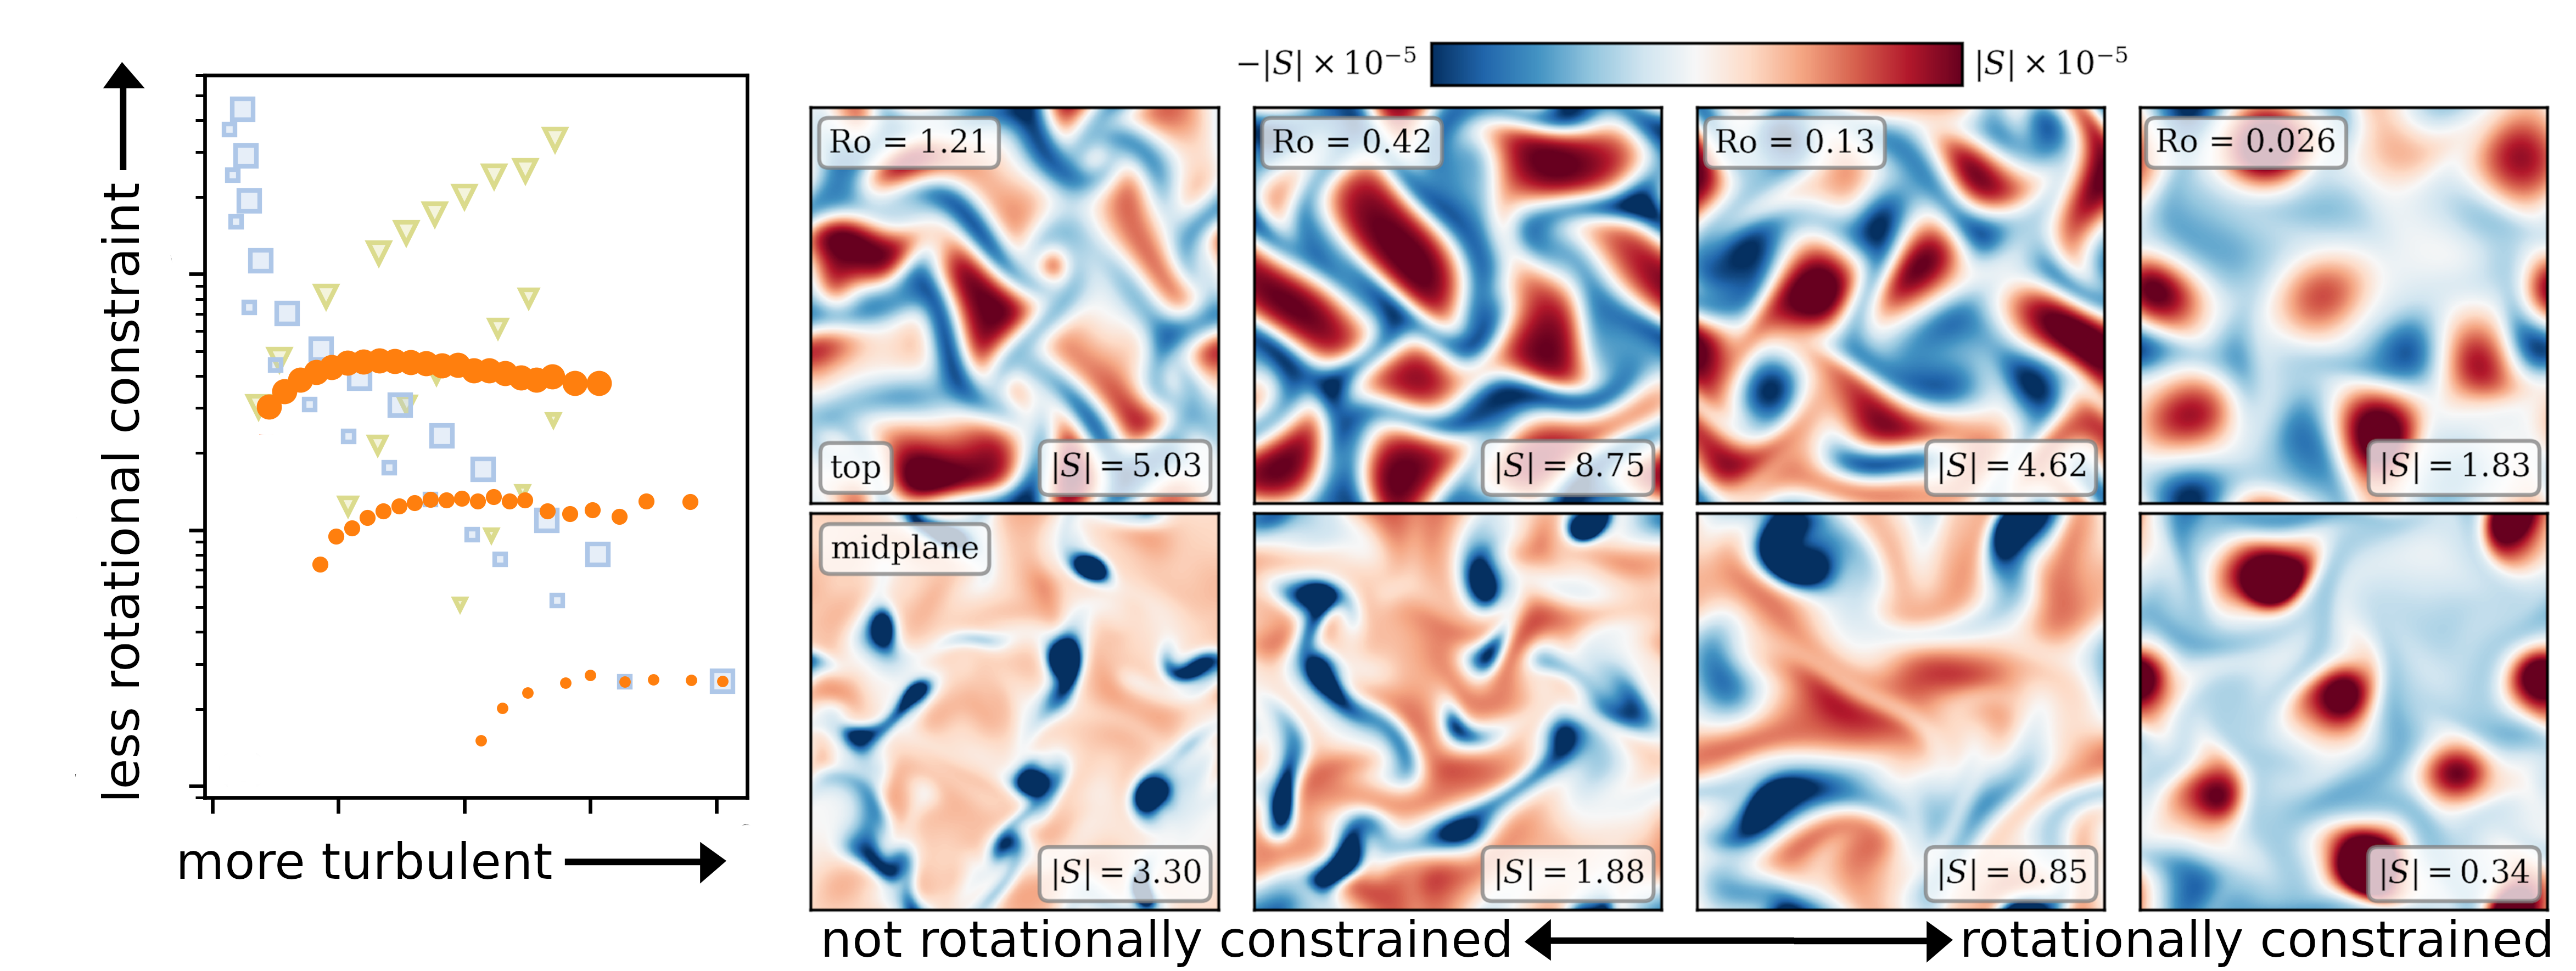
\includegraphics[width=\textwidth]{./figs/rossby_plot.png}
    \caption{(left, Fig 1b of \citet{anders&all2019}) The degree of rotational constraint is difficult to predict as a function of turbulence in convective simulations.
	Along traditional paths through parameter space (green triangles and blue squares), rotational constraint varies strongly as a function of turbulence.
	However, when our newly discovered ``predictive Rossby number'' is held constant (orange circles), the degree of rotational constraint can be held constant while turbulence is increased.
	(right eight panels, Fig. 2 of \citet{anders&all2019}) As rotational constraint increases (from left to right), traditional granular convective patterns give way to quasi-two-dimensional vortical columns of convection with very little difference between the top of the atmosphere and the atmospheric midplane (top row vs. bottom row).
	Rotational constraint modifies convective dynamics, so simulating in the proper rotational regime that reflects the Sun or another star being studied is crucial.
	\label{fig:rossby_plot} }
\end{figure*}

In solar-like stars, the strongly stratified convective zone overlies a stable interior radiative zone.
In the Sun, the radiative-convective boundary (RCB) is characterized by a transition from moderate instability to strong stability.
Now that downflows are considered a crucial element of stellar convection, it is crucial to understand how these downflows interact with the RCB.

Helioseismic measurements suggest that the RCB is thin -- roughly 5\% of a pressure scale height at the base of the convection zone, or 1\% of a solar radius \citep{basu1997}.
However, dynamics in simulations rarely achieve such a thin RCB, often times producing RCB thicknesses which are too thick or too thin by up to an order of magnitude \citep[see e.g.,][]{hotta2017, kapyla2018}.
This suggests that simulations of stellar convection are in the wrong stiffness regime \citep{brummell&all2002, couston&all2017}.
Furthermore, magnetism can appreciably alter deep velocity magnitudes, which can in turn affect RCB thicknesses \citep{hotta&all2015}.
It is widely thought that dynamics in the RCB are a critical ingredient in generating the solar dynamo and magnetic field, and so understanding the effects of a too-thick or too-thin RCB is crucial.
I propose studying how the stiffness of the RCB, which determines how hard of a ``wall'' convective motions hit at that interface, affects the transport of angular momentum and magnetic fields into the radiative zone by downflows.

I will only conduct these simulations in flow regimes where downflows can feasibly transit the solar convection zone, as determined by Task A.
In those regimes, the goal of this task is to determine how angular momentum and magnetism are pumped into the RCB as a function of RCB stiffness.

\paragraph{Task B.1: The critical magnetic field}
\label{sct:taskB1}
Convection in the presence of a strong magnetic field will have dynamics which are strongly affected by that field.
Similarly, a weak magnetic field will not noticeably affect convective motions.
Observationally, one would expect stars with more vigorous convection will have a higher critical field strength, and hotter stars will likely have more vigorous convection and higher critical field strengths.
Unfortunately, the mapping of this intuition to simulations is not straightforward, and it is difficult to predict simulation flow regimes \emph{a priori}.
The goal of this task is to determine the critical field strength at which convection passes from being weakly to strongly affected by the field.

In rotating convection, an analagous argument can be made, where convection in the presence of rapid rotation is strongly affected by Coriolis forces, and this is not true in the presence of weak rotation.
During my graduate career, I indentified the critical angular velocity, analagous to the critical magnetic field I am searching for here \citep[][and Fig. \ref{fig:rossby_plot}]{anders&all2019}.
Using similar methods to this work, I will determine what the critical magnetic field strength in these mesoscale simulations.
This knowledge of the critical magnetic field and angular velocity, will enable the stellar modeling community to specify convective flow balances in evolved convective simulations with simple input parameters.

\paragraph{Task B.2: Downflow interactions at the RCB}
\label{sct:taskB2}
In this task, I will study how downflows pump angular momentum and magnetism into or across the RCB.
I will study both very stiff RCBs, which act similar to hard wall boundaries, and very soft RCBs which convective motions can easily pass through.
Using this knowledge gained in task B.1, I will study simulations of convection in the magnetic and rotational regimes where task A revealed that downflows could transit the full convection zone.

\citet{tobias&all1998} showed that convective motions can effectively pump magnetic fields across soft RCBs in certain parameter regimes.
Here I will extend that work  to determine if magnetic fields and angular momentum are capable of being pumped into stiff RCBs by convective motions.
It is widely believed that shearing motions in the solar RCB are a critical piece of the solar dynamo, but observations \citep{basu1997} suggest that the solar RCB is stiff.
If convective motions are not able to pump magnetic fields into a stiff RCB, then a different mechanism must be responsible for generating new magnetic fields.
Furthermore, a stiff RCB could potentially insulate the solar radiative interior from convectively-driven angular momentum transport, which could help explain why the solar differential rotation profile gives way to a uniformly rotating interior beneath the RCB.

\paragraph{Task C: Global studies in relaxed atmospheres}
\label{sct:taskC}
The capstone project of my postdoctoral studies will study convection at the largest scales: global spherical simulations of rotating magnetoconvection.
The tools to perform these simulations in Dedalus already exist \citep{lecoanet&all2018} and have been tested.
One major barrier to performing global simulations is that they are costly, and some of these costs are unavoidable: highly resolved, turbulent simulations necessarily take small timesteps, and therefore simulation times are very long.
However, some of the expense of these simulations is often time wasted waiting for the atmospheric structure and mean flows to converge to an equilibrium state.
For example, the thermal structure of the Sun is thought to evolve over its Kelvin-Helmholtz timescale of $10^7$ years, which is significantly longer than its convective overturn time of five minutes at the solar surface, although still much shorter than its main sequence lifetime \citep{anders&all2018}.
As simulations approach the turbulent regime of stars, relaxation and dynamical timescales become extremely disparate, and in general numericists must choose between having state-of-the-art turbulence or converged, statistically equilibrium dynamics -- but not both.
During this third task, I will develop, test, and utilize a community tool which effectively establishes mean flows and evolves atmospheric structures by taking much larger timesteps than those of convection.
By doing so, I will enable global dynamo simulations which are both in thermal equilibrium and exhibiting state-of-the-art turbulence.

During my graduate career, I studied a mechanism for accelerating the long thermal relaxation timescale in convective systems \citep{anders&all2018}.
In this work, we discovered that a tool like the one I am proposing here can be feasibly implemented and tested for accuracy.
While studying turbulent flows, we found that our tool reached a relaxed state using an order of magnitude fewer computational resources than when waiting for a standard thermal relaxation timescale.
These speedups make achieving thermal relaxation in state-of-the-art simulations feasible.

\paragraph{Task C.1: Accelerated evolution of global simulations}
\label{sct:taskC1}
During my postdoctoral studies, I will extend my accelerated evolution method to the evolution of thermodynamic and angular momentum profiles in global simulations.
The development of this extension will be grounded in understandings gained in tasks A and B.
In particular, task A will inform which terms in the equations importantly adjust the mean field in certain regimes, and task B will inform how to implement this technique near RCB-like interfaces.
As I did in \citet{anders&all2018}, I will verify that this method produces the same results as a long relaxation in modest parameter regimes to build trust in the method.
This module will be made public, and will be designed so as to flexibly interact with arbitrary simulation data so that users of codes beyond Dedalus can benefit from the computational speed-ups of this tool.

\paragraph{Task C.2: Relaxed simulations of the solar dynamo}
\label{sct:taskC2}
I will study simulations of the interior solar convection zone in regimes where flows feel the effects of both rotation and magnetism, using the knowledge from task B.1 to determine how to set up such simulations.
Using the tool developed in task C.1, I will accelerate the evolution of these simulations.
I am predominantly interested in the relaxed differential rotation profiles that appear as a function of rotational constraint, and how these differential rotation profiles affect the time evolution of the magnetic dynamo.
In most modern dynamo simulations, the evolution of magnetic fields are measured during the relaxation process, and it is possible that the time-dependent dynamo behavior of the simulation is strongly influenced by the underlying evolution of the mean state.

While these simulations will be largely targeted in the solar context, the accelerated evolution tools which will be developed and tested here could have great benefits for asteroseismic research.
Recently, \citet{jorgensen&weiss2019} coupled three-dimensional, global simulations with 1-dimensional stellar structure tools in order to more accurately produce stellar structure profiles to great success.
The fast equilibration of angular momentum and thermal profiles described here is essentially equivalent to taking timesteps which superstep the convective motions, similar to those taken in any one-dimensional stellar structure model.
Put simply, these accelerated evolution techniques would be a first step to enabling a generalized coupling of 1-dimensional stellar structure codes with realistic statistics from converged global convection.
Future asteroseismic inversions will then benefit from stellar structure models which are influenced by three-dimensional convection including complicating effects like magnetism and rotation.

\paragraph{Computational Feasibility}
\label{sct:feasibility}
Tasks A-C are arranged logically from smallest to largest scales, and also from least to most computationally expensive.
Based on the work in \citet{anders&brown2017, anders&all2018, anders&all2019, andersLB2019}, Dedalus takes $\mathcal{O}(10^3)$ cpu-sec per iteration for a run with a grid resolution of 384$^3$ on a system comparable to NASA Pleiades.
Task A runs of thermals will take $\mathcal{O}(10^4)$ iterations each, while turbulent runs in tasks B and C will take $\mathcal{O}(10^6)$ iterations each.
Laminar thermal simulations thus cost roughly 5000 cpu-hours each, while turbulent thermals cost roughly $10^5$ cpu-hours each.
State-of-the-art simulations in tasks B and C will cost roughly $10^6$ cpu-hours each.
The projects described here total 5-10 million cpu-hours per year in tasks B and C, with less (2-3 million cpu-hours) in the first year while thermals are being studied.

The computational cost of task A should be feasible to obtain on Northwestern's 11,800-core Quest supercomputer.
In order to increase my access to computational resources and to allow for larger scale runs in tasks B and C, I will leverage my AAPF fellowship and apply for time on NSF XSEDE resources such as Stampede2, Comet, or Bridges.


\paragraph{Collaborative studies at CIERA}
\sectionmark{CIERA}
\label{sct:ciera}
Northwestern university, and specifically the Center for Interdisciplinary Exploration and Research in Astrophysics (CIERA), is the perfect location for me to carry out the work proposed here.
Dr. Daniel Lecoanet, who will be my primary advisor and collaborator, is one of Dedalus' founders.
His expertise using Dedalus and his past work on thermals \citep{lecoanet&jeevanjee2019, tarshis&all2018}, convection \citep{lecoanet&quataert2013, lecoanet&all2014, couston&all2017}, rotating convection \citep{couston&all2019}, and global simulations \citep{lecoanet&all2018} make him excellently qualified to advise me on the projects proposed here.
Furthermore, I have already published a paper on thermals in close collaboration with Dr. Lecoanet \citep{andersLB2019}, so task A will serve as an excellent transition project into my postdoctoral studies on my arrival.
In addition to Dr. Lecoanet, Dr. Yoram Lithwick would be an excellent partner for collaboration due to his past work on rotating convection \citep{BDLithwick2014} and his continuing collaborations studying careful and numerical problems in fluid disks \citep{LDLithwick2019} and planetary systems \citep{hadden&lithwick2018}.
CIERA houses many experts in computational fluid dynamics beyond Drs.~Lecoanet \& Lithwick, such as Profs.~Sasha Tchekhovskoy \& Claude-Andre Faucher-Giguere.
I look forward to joining the astrophysical fluid dynamics group at CIERA where I will have many opportunities to discuss and develop new numerical techniques, strategies, and applications across astrophysics.


Furthermore, in addition to the focused educational and outreach projects described below in section \ref{sct:broader_impacts}, CIERA will provide me with numerous small scale opportunities to participate in public outreach.
CIERA's Astronomy on Tap program as well as its CIERA Astronomer Evenings provide bite-sized and accessible ways to interact with the public.
Dearborn Observatory's observation tours are very similar to the public open houses I helped host at CU Boulder's Sommers-Bausch observatory.
The state-of-the-art Adler planetarium also provides similar opportunities such as its \emph{`Scopes in the City} program or its Space Visualization Lab astronomy conversations.


\section{Broader Impacts}
\sectionmark{Broader Impacts}
\vspace{-6pt}
\label{sct:broader_impacts}

\paragraph{Improving physics education outcomes through partnerships between pedagogical and scientific experts}
High schools in the greater Chicago area are failing to properly educate children, particularly in the sciences.
These schools perform poorly on standardized tests, with recent scores showing roughly only 40\% of high schoolers being considered proficient on Illinois' Science Assessment.
Furthermore, there are documented trends which show that low test scores are highly correlated with the degree of poverty of students in these schools.
These trends are troubling, but affecting these outcomes from a university position, or from the outside, is difficult.
While single-day university outings to schools are newsworthy, there is no evidence that such programs have lasting effects on educational outcomes.
On the other hand, a ``teach-the-teacher'' method of improving educational outcomes at the high school level has been shown to have some success.
However, the success of such programs requires the buy-in of those teachers, and therefore should offer them opportunities to engage and contribute meaningfully.
(Some research on inefficacy of college teaching of traditional lectures)

Many high school physics teachers are not necessarily experts on physics content, and could benefit from collaborative curriculum design with the consultation of experts (e.g., graduate students at CIERA).
Likewise, many expert astrophysicists and physicists are not experts on teaching pedagogy, and could achieve higher learning outcomes at the university level during their careers through the implementation of pedagogically-informed course design.
I propose the creation of a workshop series during which graduate students and local high school teachers partner to collaboratively build pedagogically- and scientifically- sound teaching modules that can be used in high school classrooms across the Chicago area and the nation.
On a small scale, teach young career scientists some basics of teaching pedagogy while also improving the content knowledge of teachers.
On a larger scale, this program will produce well-informed, bite-sized teaching modules which can be used widely in high schools, and will leverage connections and input from high school teachers to ensure that these modules are actually used in the classroom.

\paragraph{Workshop and collaboration development}
\label{sct:development}
Participation from educators will be crucial for the success of the program proposed here.
I will partner with local organizations such as Physics Northwest, the Illinoise State Physics Project (ISPP), and the Chicago Section of the American Association of Physics Teachers (CSAAPT).
Physics Northwestern's monthly meetings, ISPP's quarterly meetings, and CSAAPT's biannual meetings will be excellent venues in which to advertise the program and build a professional network of interested educators in the Chicago area.
Furthermore, CIERA's \emph{Reach for the Stars} program, a GK-12 program, has partnered with many local area high schools over the past decade and will serve as an excellent in-house link to this audience.
In addition to working with local high school educators through these avenues, I will reach out to experts in Northwestern University's School of Education and Social Policy to enlist their assistance in the development of my workshop series.

While building up these cross-disciplinary collaborations, I will work alongside Michelle Paulsen, CIERA's Director of Education, Outreach, and Communications Programs, to develop my workshop series.
Michelle has experience as a high school physics teacher and has been the chair of a large suburban high school's science department.
Furthermore, Michelle has been instrumental in the creation of CIERA's RCTP program, which develops the presentation skills of young career scientists and includes cross-disciplinary collaborations and a ten-week workshop series similar to the one I propose here.
This workshop series will take place during the summer quarter, at a time when high school educators and graduate student schedules are not constrained by the school year.

The workshops will consist of lecture portions in which professional educators teach the scientists about modern pedagogical techniques as well as collaborative small group work.
These small groups, each of which contains at least one scientist and one educator, will develop--or iterate upon--a single course module which can be used in high school classrooms.
The topic of this course module will be specified by the educator using a Next Generation Science Standards (NGSS) disciplinary core idea in physics which their students struggle to learn, and which they feel they could improve with input from an expert in the field.
During the development of each course module, an NGSS scientific practice, such as planning and carrying out investigations, will also be chosen by the group to incorporate into the module so that students have opportunities to participate in scientific practices as well as learn scientific ideas.
The work completed by each group during each workshop session will be guided by the overarching workshop structure, and in general the lecture portion of the workshop will present the daily task and evidence that supports the importance of that task.
By the end of the 10-week workshop series, with only one or two meetings a week for a couple hours a piece, a carefully constructured, scientifically sound class module will be constructed by each group.

In addition to naturally being taught in the classrooms of the teachers who participate in this workshop series, we will work to ensure further distribution of these modules.
In my later years at CIERA, in addition to using connections with Physics Northwestern, ISPP, and CSAAPT to foster educator excitement in this program, I will use these avenues to advertise the specific modules that have been created.
They will be made publically available on the American Association of Physics Teachers online ComPADRE system, which stores resources for physics and astronomy educators and is publically available.
These modules will also be made available on CIERA's website, just as products from current programs like Reach for the Stars are.

While the capstone of this workshop series for educators will be the production and use of these modules in their own classrooms, graduate students and postdocs do not have classes of students to return to with this content.
Fortunately, CIERA has a close connection with the Chicago Public Library system, and CIERA graduate students are already running data science clubs for interested area high school students.
I will work with the library, CIERA, and these data science clubs to create a venue where the graduate students can teach these modules to interested students.


\paragraph{Summary}
In short, this workshop series will partner CIERA's science experts (graduate students) with local pedagogical experts (high school teachers) to teach science experts pedagogical principles while also producing widely-used teaching modules.
This series will have the specific aims of:
\begin{enumerate}
\item Exposing interested graduate students at CIERA to best practices in teaching pedagogy, and providing those students with a teaching experience.
\item Improving high school educator understanding of a topic they struggle to teach.
\item Connecting university scientists with teachers and teaching organizations in the greater Chicago area to create lasting partnerships between scientific and pedagogical experts.
\item Creating and distributing bite-sized teaching modules appropriate to the high school level which simultaneously teach core ideas and scientific practices, as defined by Next Generation Science Standards (NGSS).
\end{enumerate}
This program aligns with NSF broader impact goals in a couple of ways.
First, it improves STEM educator development at two levels: young career scientists (graduate students) and high school educators.
Second, it widely increases public engagement with authentic science at the high school level through the wide deployment of these modules.




\section{Personal career growth and development}
\label{sct:personal_growth}
During my graduate career I participated twice in the University of California Santa Cruz's Institute for Scientist and Engineering Educators Professional Development Program (UCSC ISEE PDP), an NSF-funded program during which early career scientists spend roughly 100 hours learning the basics of teaching pedagogy while developing and teaching an authentic STEM inquiry activity.
I further spent three years as a graduate student administrator with the CU-STARs group (University of Colorado Science Technology and Astronomy RecruitS).
CU-STARs is a combined ``outreach'' and ``inreach'' program with the dual aims of increasing STEM engagement for students at underserved, rural schools across Colorado while decreasing attrition of underrepresented groups in CU Boulder's Astrophysical and Planetary Sciences department.
On top of these activities, I was a co-instructor of record for an introductory Python programming course two years ago, and my co-instructor and I completely redesigned the course curriculum before we taught the course.
These experiences have greatly informed the design of the programs presented below, and have provided me with the tools to succeed at implementing these programs.

My graduate career and the experiences within it have given me confidence that I enjoy teaching as much as research, and so my eventual career goal is to become a professor at the university level.
By developing the course proposed in section \ref{sct:inquiry_class}, I will get to continue to hone my own course design and teaching skills while also providing many early career scientists an opportunity to interact with teaching in a substantial way.
Through my outreach experience in CU STARs, I have an understanding of how to interact with high school programs and teachers, which will be necessary for the development of my course in section \ref{sct:inquiry_class}.
Furthermore, one of my many roles as a graduate student administrator in STARs was to mentor undergraduate students, and this experience has laid the groundwork for my desire to set up the mentoring program described in section \ref{sct:mentoring}.
I know that in addition to research duties, being a professor includes a great deal of teaching, departmental service, and collaboration with university institutions.
These proposed programs will help me to continue to develop as a teacher, as a negoatiator, and as an active contributor to a healthy departmental culture.

%\section{Summary and Perspectives}
%\vspace{-6pt}
%Observations of pulsating stars are becoming plentiful, and asteroseismic processing of those observations requires models which depend upon simple studies of convection.
%However, observations of the Sun have revealed that our parameterizations of convection do not adequately describe this complex process in the stellar and solar context.
%Numerical simulations at all scales and all levels of complexity have been useful tools for building theory and understanding or reproducing observations.
%Modern simulations often focus on overly complex systems, and here I propose simulations at both small and large scales which sequentially build upon and inform one another.
%
%The simulations proposed are necssary and timely.
%As continued observations pour into our databases from current and future missions, it is crucial that we do not allow the theoretical pieces of observational pipelines to be neglected.
%Current convective models cannot explain the Convective Conundrum and the combined effects of downflows, rotation, and magnetism is unclear and has not been well explored.
%Furthermore, at a time when simulations are increasingly being treated as obervations, the development of tools such as those in Task C which help ensure that convective models more accurately reflect the physics at work in stars is crucial.
%
%The fundamental problems presented here are of broad scientific interest, but are specifically topics of NSF investigation, as evidenced by the NSF's support for the DKIST telescope which will soon come online.
%The collaborative studies centered at CIERA will address the following key questions:
%\begin{itemize}
%\vspace{-9pt}
%\item Is the Sun in a regime where entropy rain is its dominant convective process and in which rotation and magnetism do not prevent this mechanism from occuring?
%\vspace{-9pt}
%\item Is the stability of the RCB important in driving the solar dynamo and the Sun's latitudinal differential rotation profile?
%\vspace{-9pt}
%\item What rotational regime is the Sun in, and what can we learn about dynamo evolution in that regime?
%\vspace{-9pt}
%\end{itemize}
%
%As stated previously, the work designed as Task A will occupy my research time during my first year while I lay the groundwork for my mentorship program and course on teaching pedagogy.
%Task B will occupy my time during my second year, while I launch my mentorship program, teach my class for the first time, and work to improve both of these programs.
%I will cap off my time at CIERA with task C while I work to ensure that the programs and classes that I set up smoothly transition to new leadership when I leave so that future students can continue to benefit from these programs.
%

\newpage
\AtBeginShipout{%
\AtBeginShipoutDiscard
}
\setcounter{page}{1}
\nosection{References}
\bibliographystyle{apj_title}


%\newpage
%\bibliographystyle{apj_title}
\bibliography{biblio}
\end{document}
